\documentclass[a4paper,11pt]{article}
\usepackage[T1]{fontenc}
\usepackage[polish]{babel}
\usepackage[utf8]{inputenc}
\usepackage{lmodern}
\usepackage{pgfplots}
\usepackage{graphicx}
\graphicspath{ {./images/} }
\selectlanguage{polish}
\usepackage{geometry}
\usepackage{listings}
\newgeometry{tmargin=3cm, bmargin=3cm, lmargin=2.5cm, rmargin=2.5cm}
\title{
	\date{18 stycznia 2020}
	\textbf{Programowanie równoległe i rozproszone}\vspace{40pt}
	\\\textit{Politechnika Krakowska} \\\vspace{40pt}
	\textup{Projekt}\vspace{25pt}
	\\\textup{Temat}\
	\\\textit{Porównanie czasów działania sieci neuronowych oraz głębokich sieci w środowiskach TensorFlow, PyTorch i Theano} \\\vspace{26pt}
	\vspace{270pt}
}
\author{
	Paweł Suchanicz,\\
	Rafał Niemczyk
}
\begin{document}
\begin{titlepage}
\maketitle
\end{titlepage}

\begin{center}
\tableofcontents
\end{center}
\newpage
\section{Wstęp}
\subsection{Opis projektu}
\paragraph{}Celem projektu było porównanie czasów działania sieci neuronowych oraz głębokich sieci neuronowych w środowiskach: TensorFlow, PyTorch oraz Theano. Czasy należało zmierzyć na CPU oraz GPU, jeśli była taka możliwość. 
\paragraph{}Pomiary czasów należało dokonać dla każdego z 4 zbiorów danych. Dlatego zbudowano 4 różne architektury sieci neuronowych. W każdym ze środowisk zbudowano te same architektury oraz zachowano te same parametry uczenia czy też funkcje aktywacji.
\paragraph{}Dodatkowo należało dokonać eksperyment w 2 wariantach:
\begin{itemize}
\item Podział na zbiór uczący i testowy (70%, 30%)
\item 10 krotna walidacja krzyżowa
\end{itemize}
\paragraph{}Aby porównanie czasów było jak najbardziej obiektywne użyto domyślnego timera udostępnionego przez Python - timeit.
\paragraph{}Aby uruchomić obliczenia sieci neuronowych na GPU należało użyć technologii CUDA. CUDA (Compute Unified Device Architecture) to architektura kart graficznych opracowana przez firmę Nvidia. Pozwala na wykorzystanie mocy obliczeniowej na kartach graficznych.
\subsection{Opis zbiorów danych}
\subsubsection{MNIST}
\paragraph{}Jest to zestaw odręcznie napisanych cyfr (od 0 do 9), który powszechnie używany jest do szkolenia różnych systemów przetwarzania obrazu oraz w dziedzinie uczenia maszynowego. Baza danych MNIST zawiera 60 000 obrazów szkoleniowych i 10 000 obrazów testowych. Wielkość każdego obrazu to 28 x 28 pikseli w skali szarości. \\
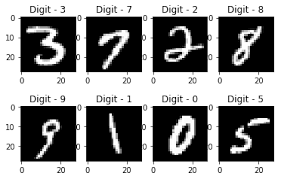
\includegraphics{MNIST}

\subsubsection{CIFAR10}
\paragraph{}Jest to zestaw zawierający 60 000 kolorowych obrazów o wielkości 32 x 32 pikseli. Obrazy przedstawiają jedną z 10 klas. Na poniższym obrazku znajdują sie klasy wraz z przykładowymi obrazami. Każda klasa zawiera 6000 obrazów. Dane treningowe składają się z 50 000 obrazów, a testowe z 10 000, czyli w danych treningowych znajduję się 5 000 obrazów jednej klasy, a w testowe 1 000. Klasy całkowicie się wykluczają.\\
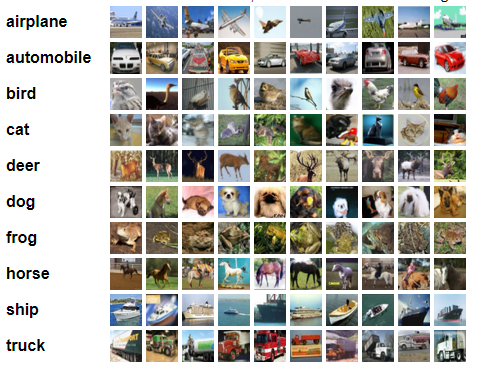
\includegraphics{cifar10}

\subsubsection{CIFAR100}
\paragraph{}Ten zestaw danych zawiera 60 000 kolorowych obrazów. Obrazy reprezentują 100 różnych klas, co oznacza, że na każdą klasę przypada 600 obrazów. Z każdej klasy wyodrębnionych zostaje 500 obrazów treningowych oraz 100 testowych. Każda z 100 klas jest przypisana do jednej z 20 superklas, czy też nadklas. Każdy obraz ma dwie etykiety. Jedną jako etykietę nadklasy i drugą jako własną. Poniżej znajduję się tabelami przedstawiająca nadklasy i klasy do nich należące.
\begin{tabular}{|c|c|}
\hline Nazwa nadklasy &Nazwy klas zawartych w nadklasie \\ 
\hline Ssaki wodne& bóbr, delfin, wydra, foka, wieloryb\\
\hline Ryby& ryba akwariowa, rekin, pstrąg, płastugi, płaszczka\\
\hline Kwiaty& storczyk, mak, róża, słonecznik, tulipan \\
\hline Pojemniki na żywność& butelka, miska, puszka, kubek, talerz \\
\hline Warzywa i owoce& jabłko, grzyb, pomarańcza, gruszka, papryka \\
\hline Urządzenia elektryczne& zegar, klawiatura, lampa, telefon, telewizja \\
\hline Meble domowe& łóżko, krzesło, kanapa, stół, szafa \\
\hline Owady& pszczoła, chrząszcz, motyl, gąsienica, karaluch \\
\hline Duże drapieżniki& niedźwiedź, lampart, lew, tygrys, wilk \\
\hline Wszystkożerne i roślinożerne & wielbłąd, szympans, słoń, kangur, bydło \\
\hline Średniej wielkości ssaki& lis, jeżozwierz, szop, skunks, opos \\
\hline Bezkręgowce& krab, homar, ślimak, pająk, robak \\
\hline Człowiek& niemowlę, chłopak, dziewczyna, mężczyzna, kobieta \\
\hline Gady& krokodyl, dinozaur, jaszczurka, wąż, żółw \\
\hline Małe ssaki& chomik, mysz, królik, wiewiórka, ryjówka  \\
\hline Drzewa& klon, dąb, palma, sosna, wierzba \\
\hline Pojazdy 1& rower, autobus, motocykl, furgonetka, pociąg \\
\hline Pojazdy 2& kosiarka, rakieta, tramwaj, czołg, ciągnik \\
\hline
\end{tabular}
\subsubsection{Letter Recognition}
\paragraph{}Dane stworzone po to, aby móc na podstawie wyświetlanych pikseli zidentyfikować jedną z 26 wielkich liter alfabetu angielskiego. Obrazy znaków zostały oparte na 20 różnych czcionkach, a każda litera w tych 20 czcionkach została losowo zniekształcona, aby utworzyć plik zawierający 20 000 unikalnych cech. Każda litera składa się z 16 cech ją opisujących. Cechy, które tworzą poszczególną literę to:
\begin{itemize}
\item letter - wielka litera (od A do Z)
\item x-box - pozioma pozycja x (liczba całkowita)
\item y-box - pionowa pozycja y (liczba całkowita)
\item width - szerokość (liczba całkowita)
\item high - wysokość (liczba całkowita)
\item onpix - całkowita liczba pikseli (liczba całkowita)
\item x-bar - średnia liczba pikseli x (liczba całkowita) 
\item y-bar - średnia liczba pikseli y (liczba całkowita) 
\item x2bar - średnia wariancja x (liczba całkowita) 
\item y2bar - średnia wariancja y (liczba całkowita) 
\item xybar - średnia korelacja x y (liczba całkowita) 
\item x2ybr - średnia x * x * y (liczba całkowita) 
\item xy2br - średnia x * y * y (liczba całkowita) 
\item x-ege- średnia liczba krawędzi od lewej do prawej (liczba całkowita) 
\item xegvy - korelacja x krawędzi z y (liczba całkowita) 
\item y-ege- średnia liczba krawędzi od dołu do góry (liczba całkowita)
\item yegvx - korelacja y krawędzi z x (liczba całkowita)
\end{itemize}
\subsection{Opis użytych frameworków}
\subsubsection{Keras}
\paragraph{}Keras to biblioteka open-suorce do sieci neuronowych napisana w pythonie. zaprojektowana, aby umożliwić szybkie eksperymentowaie z głębokimi sieciami neuronowymi. Koncentruje się na byciu przyjazną dla użytkownika. W 2017 roku, zespół Google TensorFlow postanowił wesprzeć Keras w podstawowej bibliotece Tensorflow. Keras został mianowany jako przyjazny interfejs niż samodzielna platforma uczenia maszynowego. Oferuje bardziej intuicyjny zestaw narzędzi, które ułatwiają opracowywanie modeli głębokiego uczenia niezależnie od zastosowanego zaplecza obliczeniowego. 
\paragraph{}Keras był początkowo zawarty w temacie projektu, jednak po przeanalizowaniu i wgłebieniu się w temat frameworków do uczenia maszynowego w pythonie, zrezygnowano z tej opcji. Jak już wspomniano, biblioteka świetnie spisuje się do tworzenia architektury sieci neuronowych oraz do tworzenia całych modeli wraz z parametrami uczenia i funkcjami aktywacji. Jednak obliczenia wykonywane podczas treningu sieci, wykonywane domyślnie są za pomocą biblioteki TensorFlow. Aktualnie oprócz biblioteki obliczeniowej TensorFlow, są dostepne dwie inne biblioteki: Theano oraz CNTK.
\subsubsection{Tensorflow} 
\paragraph{}Tensorflow jest biblioteką open-source. Została napisana przez Google Brain Team w celu zastąpenia Theano. Wykorzystywana w uczeniu maszynowym i głębokich sieciach neuronowych. Została wydana 9 listopada 2015 roku. Biblioteka może do działania wykorzystywać zarówno karty graficzne, procesory jak i wyspecjalizowane mikroprocesory. Biblioteka składa się z kilku modułów. W jej najniższej warstwie znajduje się rozproszony silnik wykonawczy (ang. distributed execution engine), który w celu podniesienia wydajności został zaimplementowany w języku programowania C++. Nad nią znajdują się frontendy napisane w kilku językach programowania m.in. w Pythonie oraz C++. Powyżej umieszczona została warstwa API, która zapewnia prostszy interfejs dla powszechnie używanych warstw w modelach głębokiego uczenia. Na następną warstwę składają się wysokopoziomowe API, m.in. Keras oraz Estimator API, które ułatwiają tworzenie modeli i ich ocenę. Ponad tym znajdują się przygotowane przez twórców biblioteki gotowe do użycia modele.
\paragraph{}Uważa się, że TensorFlow jest sybszy niz Theano. Jednak jest wolniejszy niz inne frameworki. Dodatkowo nie posiada zbyt dużej liczby wyszkolonych modeli. 
\subsubsection{PyTorch}
\paragraph{}Jest to open-source biblioteka do uczenia maszynowego, bazująca na bibliotece Torch. Używana do aplikacji jak przetwarzanie języka naturalnego. Opracowana głównie przez Facebook AI Research lab. Oprócz interfejsu pythona, posiada interfejs C++. Na PyTorch zbudowanych jest wiele elementów oprogramowania do głębokiego uczenia, jak Uber Pyro. Zapewnia dwie funkcje wysokiego poziomu:
\begin{itemize}
\item obliczenia tensorowe z silnym przyśpieszeniem za pośrednictwem procesorów graficznych GPU
\item głębokie sieci neuronowe zbudowane na systemie autodiff
\end{itemize}
\paragraph{}Do plusów biblioteki można zaliczyć np: wiele modułów, które można łatwo połączyć; łatwe pisanie własnych typów warstw i uruchamianie na GPU, wiele wstępnie przeszkolonych modeli. Minusami tej biblioteki są: pisanie własnego kodu treningowego, brak wsparcia.
\subsubsection{Theano}
\paragraph{}Jest to biblioteka i kompilator optymalizujący wyrażenia matematyczne. W Theano obliczenia są wyrażane przy użyciu skłądni w stylu NumPy i kompilowane w celu wydajnego działania na architekturze CPU lub GPU. Projekt typu open-source, opracowany przede wszystkim przez Montreal Institute for Learning na Uniwerstytecie w Montrealu. W dniu 28 września 2017 roku, Yoshua Bengio ogłosił: "Główny rozwój zostanie zakończony po wydaniu wersji 1.0, z powodu konkurencyjnych ofert silnych graczy przemysłowych. Wersja 1.0.0 została wydana 15 listopada 2017r. Na Theano zbudowano biblioteki głębokiego uczenia jak Keras, Lagane i Blocks. 
\subsection{Specyfikacja sprzętowa}
\paragraph{}Przy pomiarach szybkości wykonywania algorytmów wykorzystany był sprzęt w konfiguracji 
- do implementacji z wykorzystaniem CUDA.
\\Specyfikacja sprzętu:
\begin{itemize}
\item Procesor: Intel Core i7-4712MQ 4 x 2.30GHz
\item Ram: 8GB DDR3
\item System: Windows 10
\item GPU: NVIDIA GeForce 840N
\
\end{itemize}
\section{Wyniki}
\subsection{Implementacja} 
\paragraph{}W projekcie należało użyć trzech frameworków: TensorFlow, PyTorch oraz Theano. Dwa z nich, TensorFlow oraz Theano, można użyć jako backend do biblioteki Keras. Dzięki czemu dla tych dwóch frameworków stworzono cały model uczenia używając dokładnie tych samych funkcji dostępnych dzięki Keras. 
\subsubsection{Wczytanie danych}
\paragraph{}Trzy z 4 zbiorów danych zawarte są w paczkach danych udostępnionych przez Keras. Należało jedynie poprawnie wywołać odpowiednią funkcję. Podobnie sytuacja wyglądała w PyTorch, gdzie zbiory były dostępne i również należało wykonać poszczególną funkcję.
\paragraph{}Aby wczytać zbiór LetterRecognition należało użyć funkcji read-csv dostępnej w paczce Pandas. 
\paragraph{}Dane nie wymagały zbyt dużej obróbki, ponieważ nie brakowało żadnych wartości oraz były zapisane w postaci numerycznej. Podczas wczytania danych poprzez funkcję udostępnioną przez Keras, dane były domyślnie dzielone na treningowe i testowe. Jednak proporcje tych danych nie spełniały wymagań projektowych. Dlatego łączono dane i dopiero w następnym kroku dzielono je na odpowiednie proporcje lub używano do walidacji krzyżowej.
\subsubsection{Architektura sieci}
\paragraph{}Stworzenie architektury sieci w bibliotece Keras polega głównie na funkcjach udostępnianych przez bibliotekę. Jest to bardzo proste zajęcie, należy tylko odpowiednie dodawać kolejne warstwy sieci do modelu.
\paragraph{}W przypadku PyTorch sytuacja wygląda bardzo podobnie. Należy odpowiednio ułożyć warstwy sieci. Główne różnice można zauważyć w nazewnictwie.
\paragraph{}Poniżej znajdują się utworzone architektury sieci dla każdego ze zbiorów danych.\\
\begin{itemize}
\setlength\itemsep{1em}
	\item MNIST\par\par
	\begin{minipage}{\linewidth}
		\par\paragraph{}
		\centering
		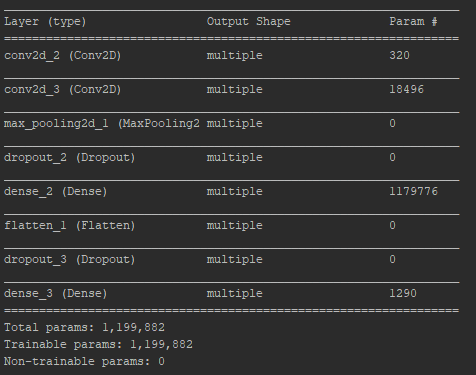
\includegraphics[width=1\linewidth]{modelMnist}
	\end{minipage}
	\begin{minipage}{\linewidth}
		\centering
		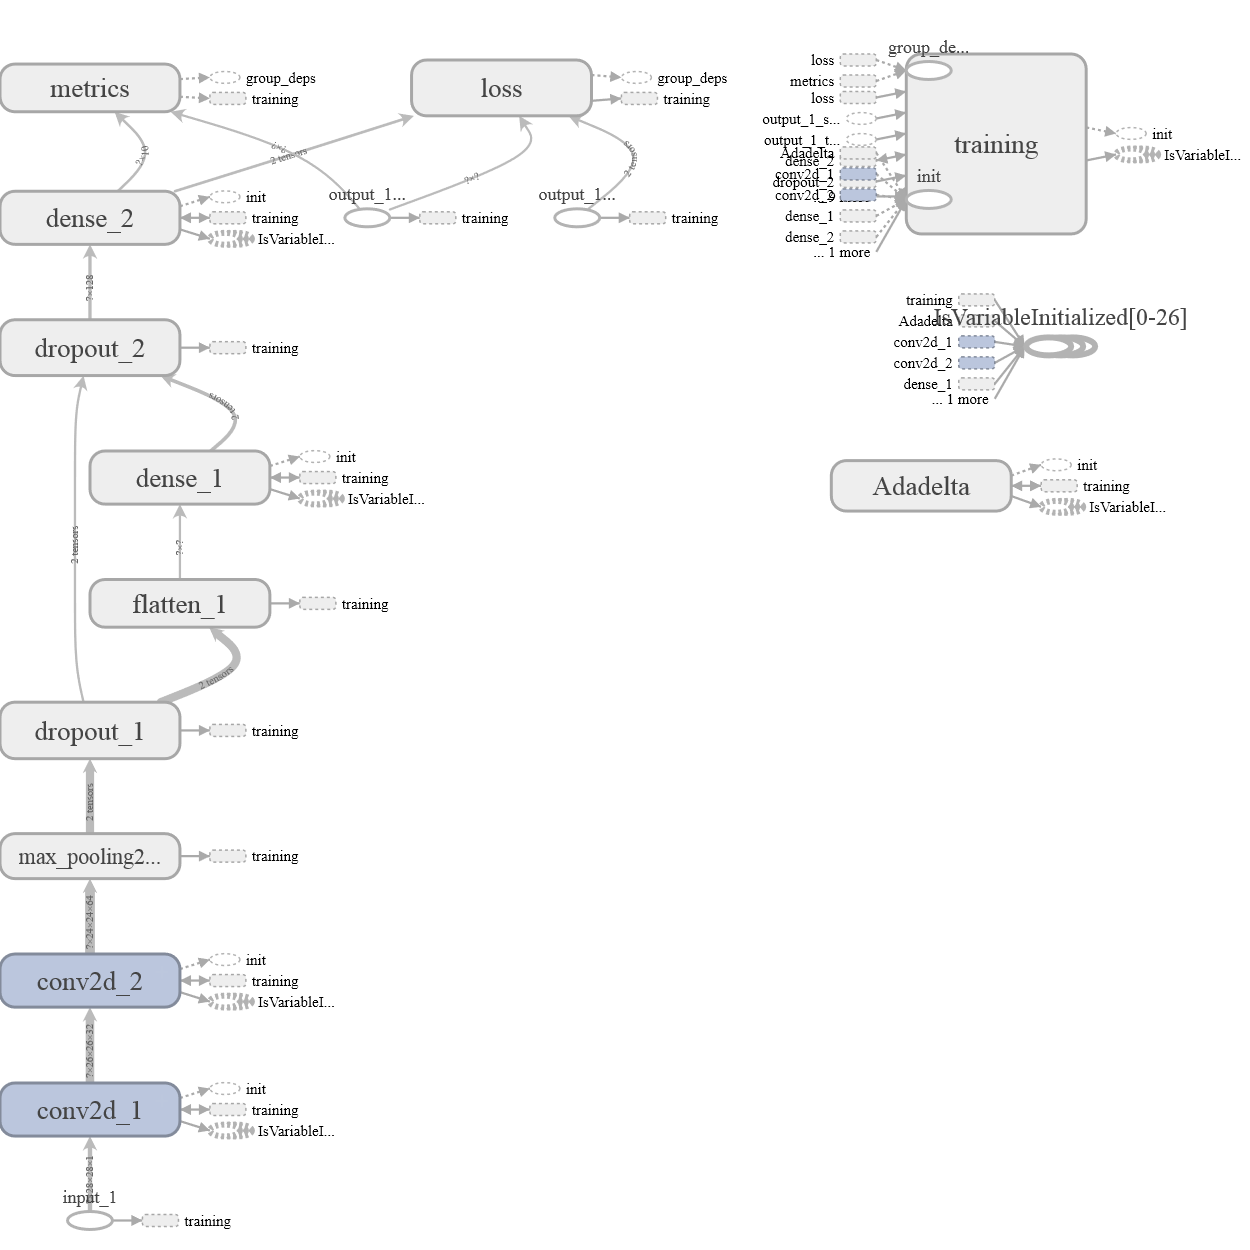
\includegraphics[width=1\linewidth]{mnist-graph}
	\end{minipage}
	
	\newpage
	\item CIFAR10\par
	\begin{minipage}{\linewidth}
		\centering
		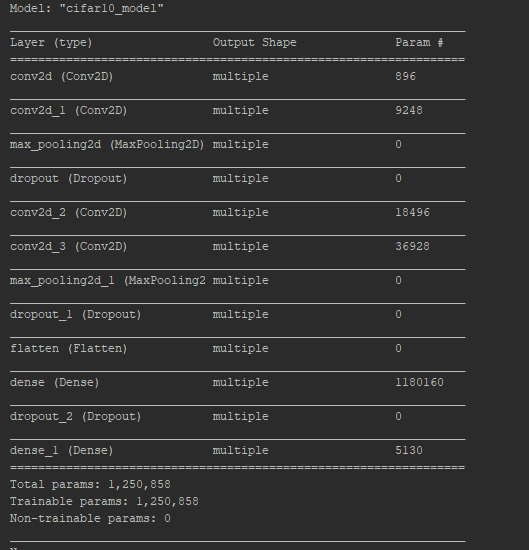
\includegraphics[width=1\linewidth]{modelCifar10}
	\end{minipage}
	\begin{minipage}{\linewidth}
		\centering
		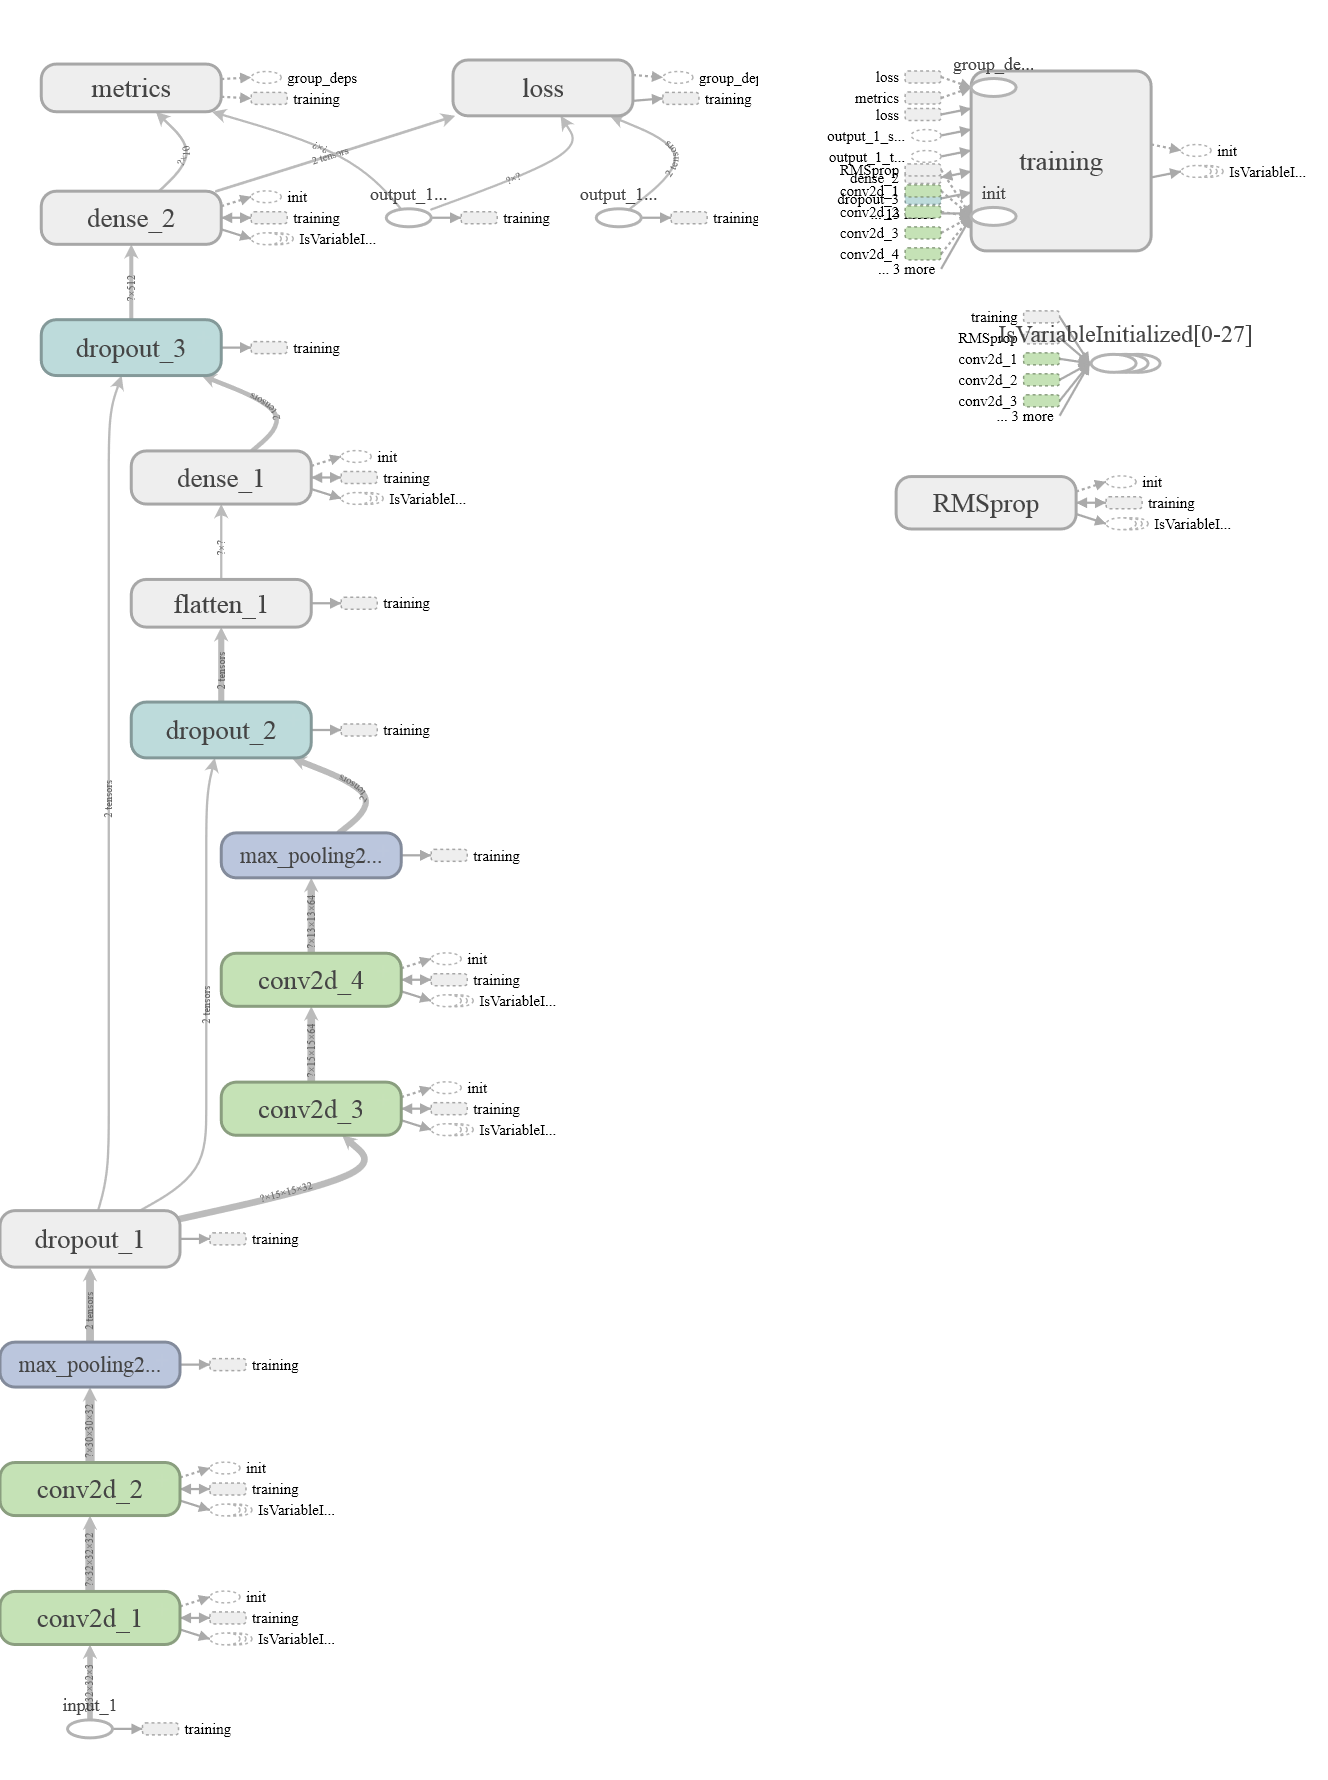
\includegraphics[width=1\linewidth]{cifar10-graph}
	\end{minipage}

	\newpage
	\item CIFAR100\par
	\begin{minipage}{\linewidth}
		\centering
		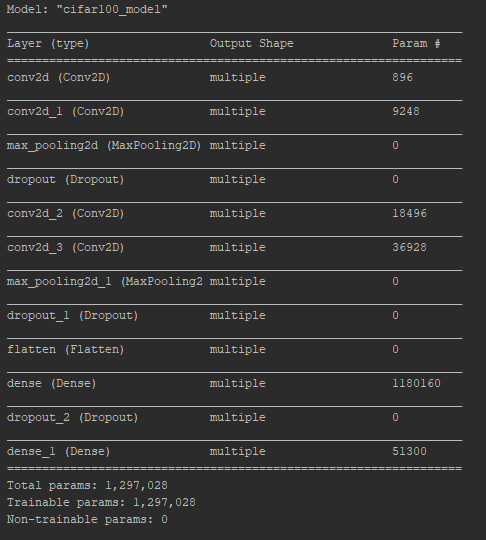
\includegraphics[width=1\linewidth]{modelCifar100}
	\end{minipage}
	\begin{minipage}{\linewidth}
		\centering
		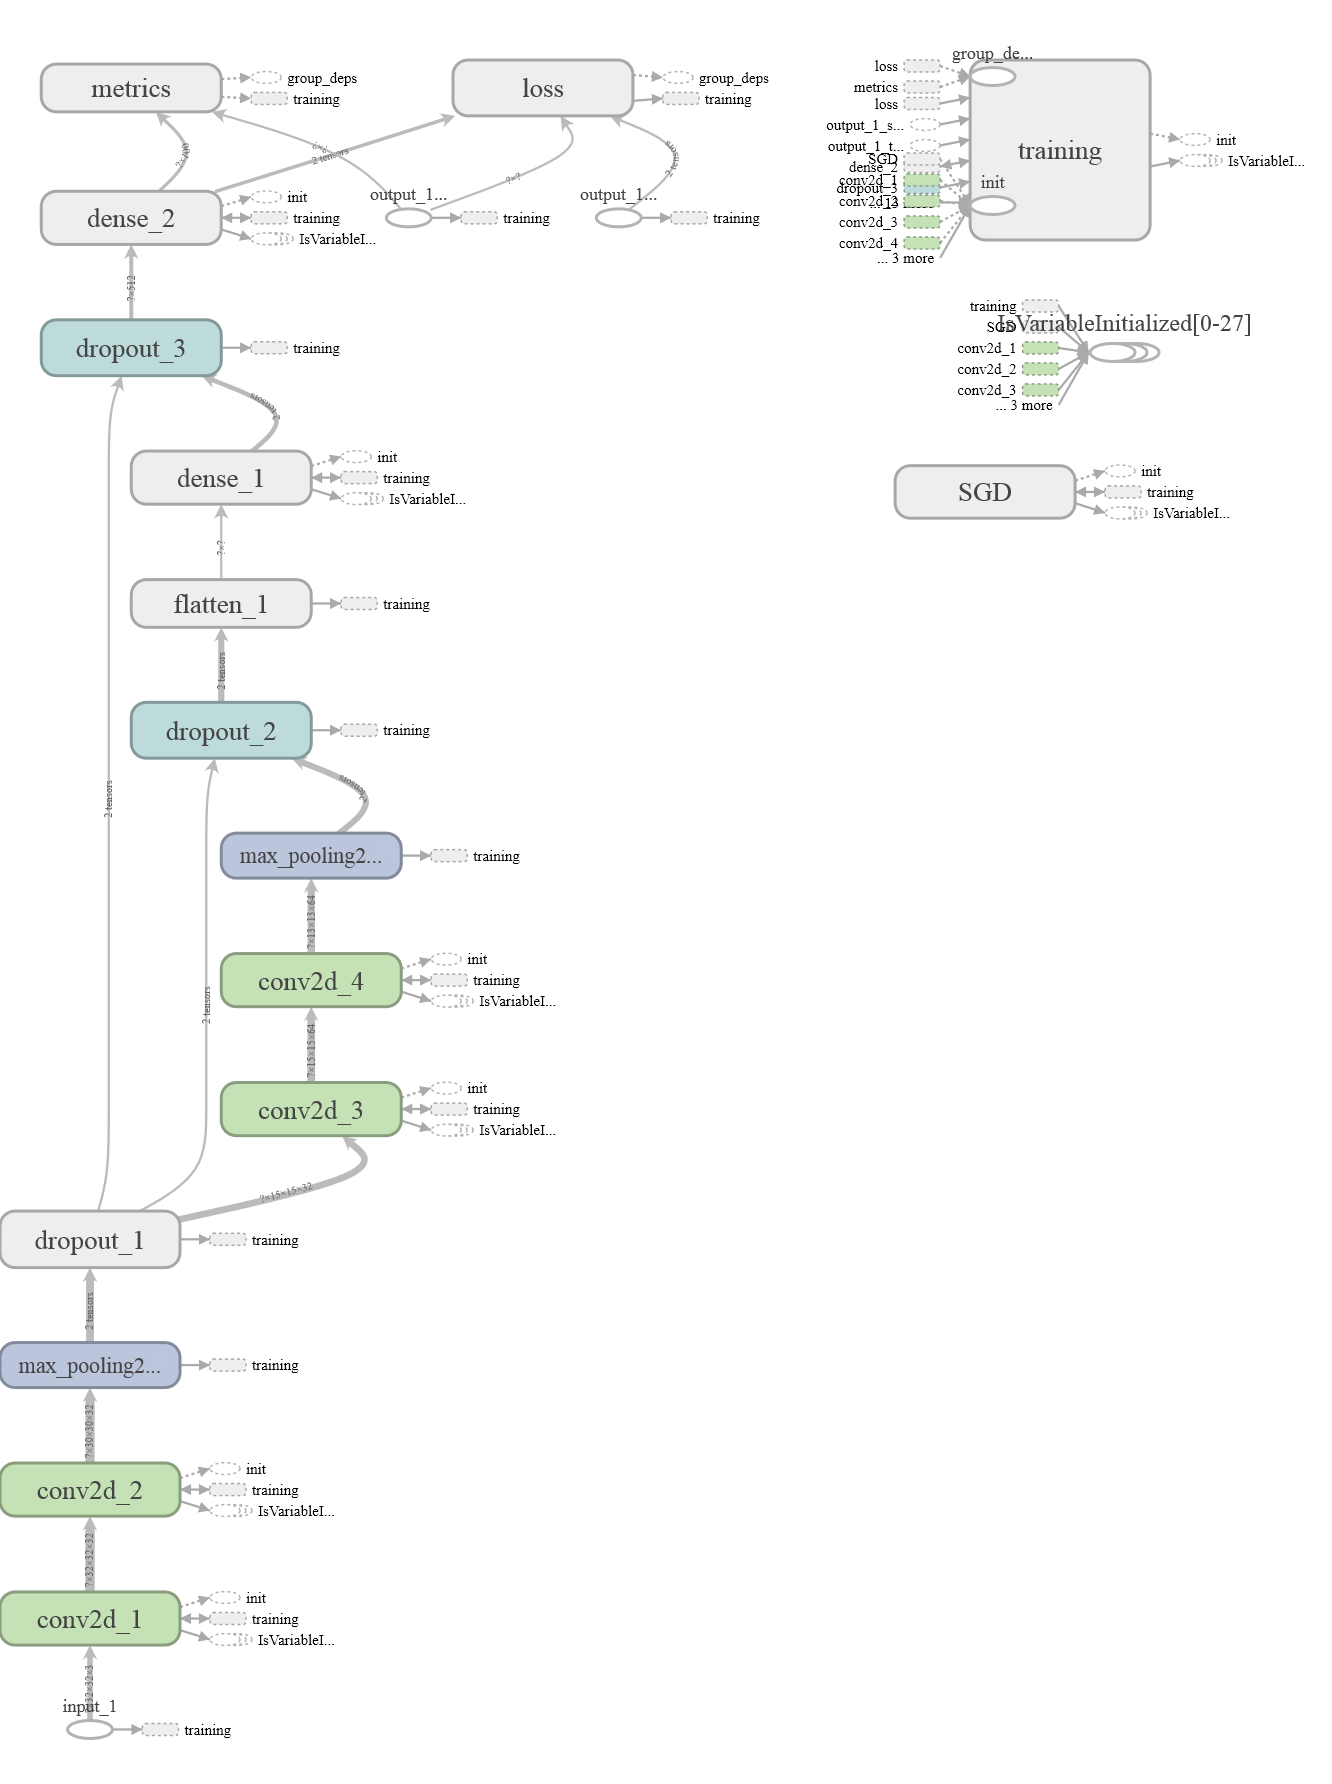
\includegraphics[width=1\linewidth]{cifar100-graph}
	\end{minipage}

	\newpage
	\begin{minipage}{\linewidth}
	\item LetterRecognition\par
		\centering
		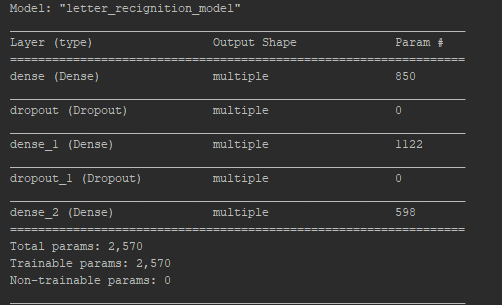
\includegraphics[width=1\linewidth]{modelLetter}
	\end{minipage}
	\begin{minipage}{\linewidth}
		\centering
		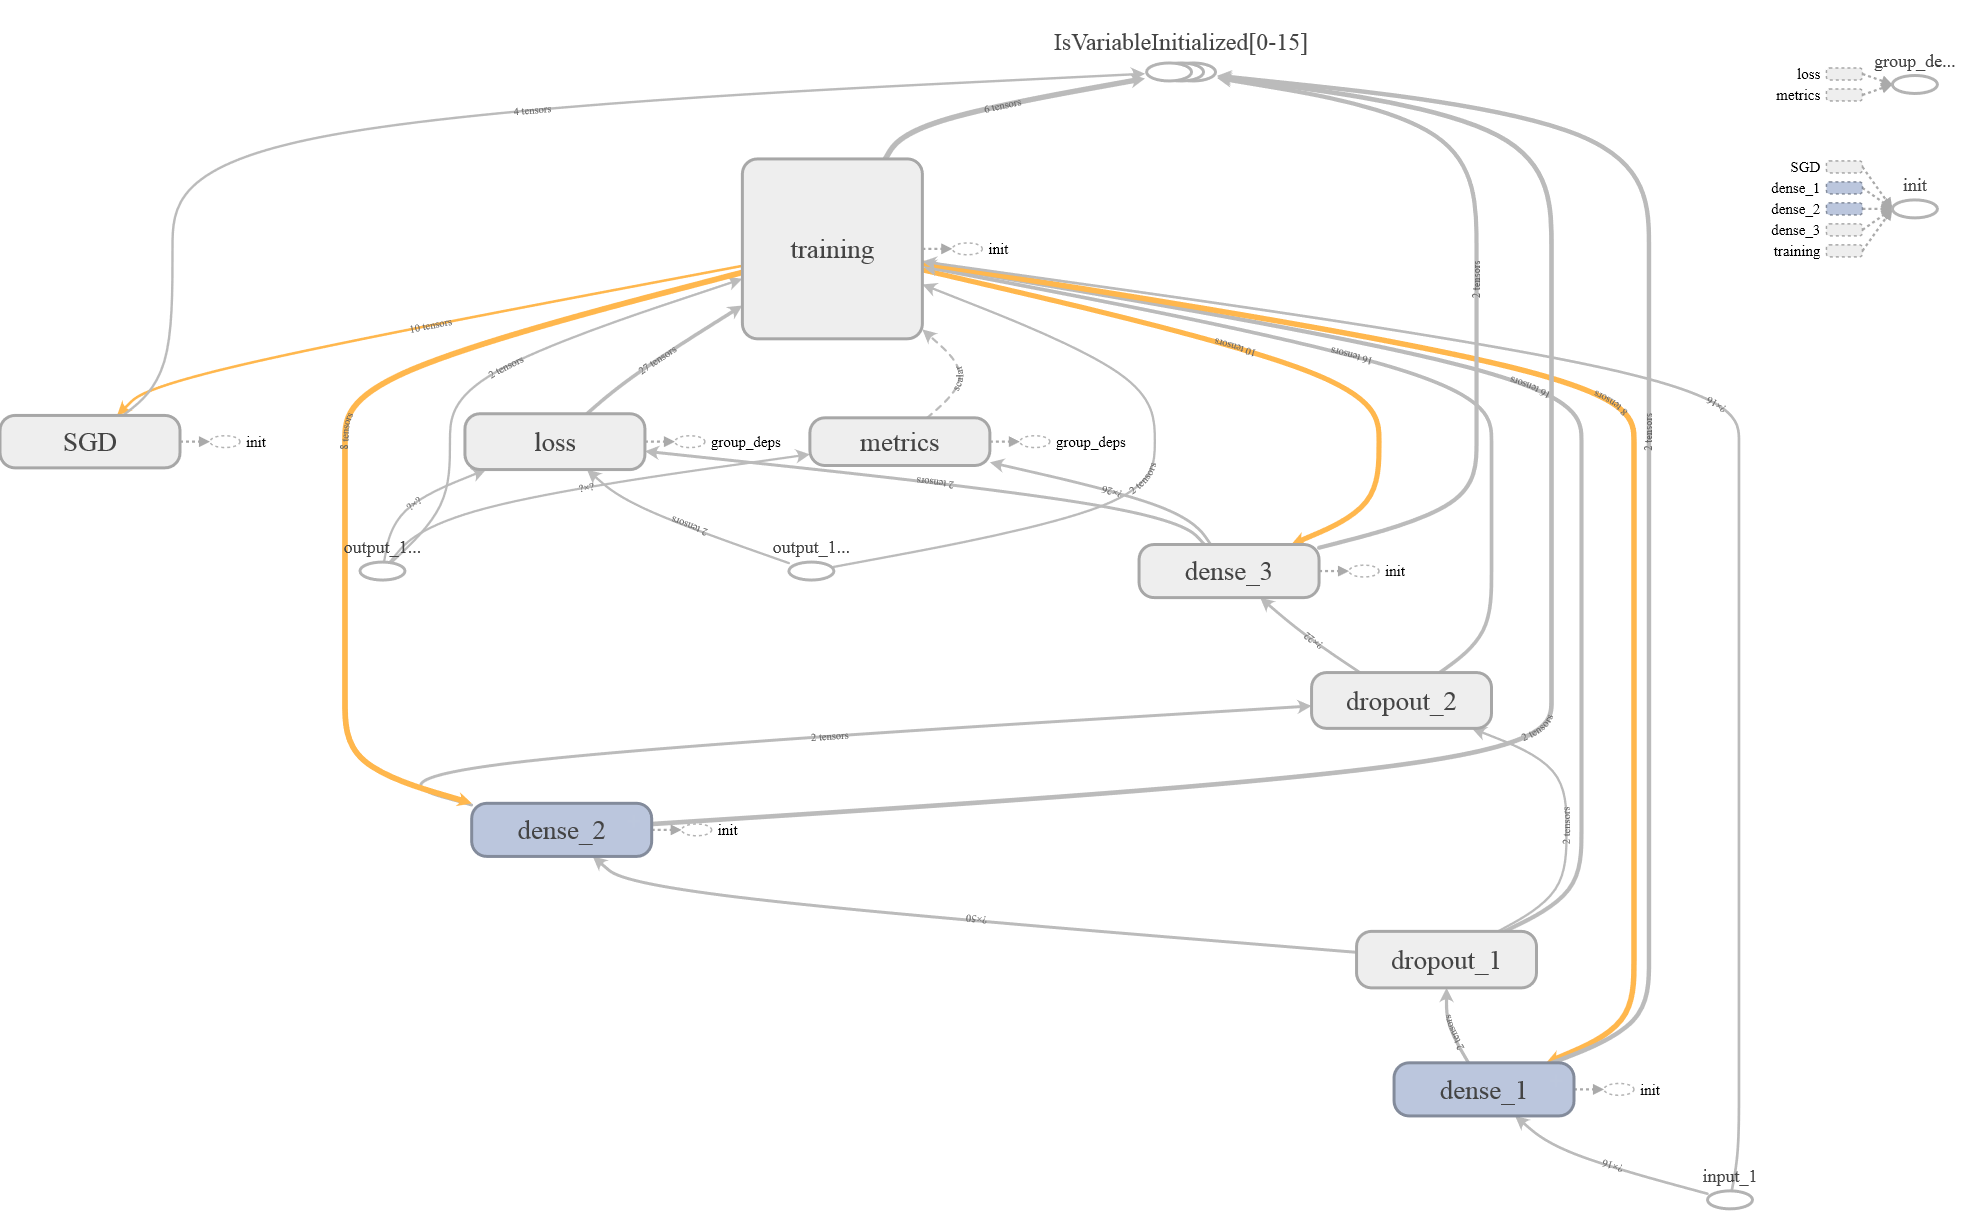
\includegraphics[width=1\linewidth]{letter-recognition-graph}
	\end{minipage}
\end{itemize}
\subsubsection{Parametry uczenia}
\paragraph{}Dla każdej architektury dobrane inne parametry uczenia, co wyszczególniono poniżej:
\begin{itemize}
\item MNIST:
\begin{itemize}
\item funkcja błędu - categorical-crossentropy
\item optymalizator  - Adadelta()
\item batch-size = 128
\item liczba epok = 12
\end{itemize}
\item CIFAR10:
\begin{itemize}
\item funkcja błędu - categorical-crossentropy
\item optymalizator  - RMSprop(learning-rate=0.0001, decay=1e-6)
\item batch-size = 128
\item liczba epok = 12
\end{itemize}
\item CIFAR100:
\begin{itemize}
\item funkcja błędu - categorical-crossentropy
\item optymalizator  - SGD(lr=0.01, decay=1e-6, momentum=0.9, nesterov=True)
\item batch-size = 128
\item liczba epok = 12
\end{itemize}
\item LetterRecognition:
\begin{itemize}
\item funkcja błędu - categorical-crossentropy
\item optymalizator  - SGD(lr=0.001, decay=1e-7, momentum=0.)
\item batch-size = 128
\item liczba epok = 300
\end{itemize}
\end{itemize}
\paragraph{}Aby zainicjalizować wagi w Keras należy użyć metody compile, natomiast w PyTorch należy przekazać funkcję modyfikującą wagi. Tworzenie optymalizatorów jest bardzo podobne w obu frameworkach.
\subsubsection{Podział danych}
\paragraph{}Wykonując zadanie zawarte w poleceniu, tzn aby podzielić dane na testowe i treningowe w proporcji 70\%{\char`\/}30\% użyto funkcji train-test-split z pakietu sklearn. 
\subsubsection{Walidacja krzyżowa}
\paragraph{}Walidacja krzyżowa jest metodą statystyczną, polegająca na podziale próby statystycznej na podzbiory, a następnie przeprowadzaniu wszelkich analiz na niektórych z nich (zbiór uczący), podczas gdy pozostałe służą do potwierdzenia wiarygodności jej wyników (zbiór testowy). K-Krotna walidacja to metoda w której oryginalna próba jest dzielona na K podzbiorów. Następnie kolejno każdy z nich bierze się jako zbiór testowy, a pozostałe razem jako zbiór uczący i wykonuje analizę. Analiza jest więc wykonywana K razy. K rezultatów jest następnie uśrednianych (lub łączonych w inny sposób) w celu uzyskania jednego wyniku. Aby skorzystać z walidacji krzyżowej użyto funkcji KFold z pakietu sklearn. 
\subsection{Porównanie wyników - CPU} 
\subsubsection{Walidacja krzyżowa}
\paragraph{}Porównanie wyników, gdy uczenie sieci uruchomiono na CPU i wykorzystano walidację krzyżową.
\paragraph{Czas wykonania}
\begin{tabular}{|c|c|c|c|}
\hline &TensorFlow & Theano & PyTorch \\ 
\hline MNIST &12089.98s &12405.71s  &23848.42s  \\ 
\hline CIFAR10 &15902.45s &19150.98s  &27867.25s  \\ 
\hline CIFAR100 &17127.30s &457762.47s  &32609.92s  \\ 
\hline LetterRec &1551.61s &1071.60s &2019.43s  \\ 
\hline
\end{tabular}
\paragraph{Test accuracy}
\begin{tabular}{|c|c|c|c|}
\hline &TensorFlow & Theano & PyTorch \\ 
\hline MNIST &82.56\% &83.86\%  &98.97\%  \\ 
\hline CIFAR10 &61.72\%  &62.95\%  &62.70\%  \\ 
\hline CIFAR100 &39.52\% &46.13\%  &43.92\%  \\ 
\hline LetterRec &69.25\% &67.60\%  &66.55\%  \\ 
\hline
\end{tabular}
\subsubsection{Podział danych 70/30}
\paragraph{}Porównanie wyników, gdy uczenie sieci uruchomiono na CPU i wykorzystano podział 70/30.
\paragraph{Czas wykonania}
\begin{tabular}{|c|c|c|c|}
\hline &TensorFlow & Theano & PyTorch \\ 
\hline MNIST &1005.69s &1928.22s  &1281.81s  \\ 
\hline CIFAR10 &1480.35s &3112.23s  &1524.95s  \\ 
\hline CIFAR100 &1551.61s &74422.8454s  &1890.53s  \\ 
\hline LetterRec &90.876s &108.85s  &154.82s  \\ 
\hline
\end{tabular}
\paragraph{Test accuracy}
\begin{tabular}{|c|c|c|c|}
\hline &TensorFlow & Theano & PyTorch \\ 
\hline MNIST &81.26\% &98.96\%  &98.61\%  \\ 
\hline CIFAR10 &57.63\%  &57.27\%  &48.75\%  \\ 
\hline CIFAR100 &39.54\% &44.21\%  &36.34\%  \\ 
\hline LetterRec &3.2\% &3.68\%  &48.82\%  \\ 
\hline
\end{tabular}
\subsection{Porównanie wyników - GPU} 
\subsubsection{Walidacja krzyżowa}
\paragraph{}Porównanie wyników, gdy uczenie sieci uruchomiono na GPU i wykorzystano walidację krzyżową.
\paragraph{Czas wykonania}
\begin{tabular}{|c|c|c|c|}
\hline &TensorFlow & Theano & PyTorch \\ 
\hline MNIST &3623.60s &7587.83s  &4026.90s  \\ 
\hline CIFAR10 &4558.62s &9226.08s  &3876.99s  \\ 
\hline CIFAR100 &4264.93s &10257.84s  &3907.12s  \\ 
\hline LetterRec &1905.68s &1451.61s  &5090.07s  \\ 
\hline
\end{tabular}
\paragraph{Test accuracy}
\begin{tabular}{|c|c|c|c|}
\hline &TensorFlow & Theano & PyTorch \\ 
\hline MNIST &83.34\% &98.94\%  &99.08\%  \\ 
\hline CIFAR10 &63.10\%  &62.60\%  &62.53\%  \\ 
\hline CIFAR100 &37.09\% &36.43\%  &44.41\%  \\ 
\hline LetterRec &67.46 \% &72.25  &50.15\%  \\ 
\hline
\end{tabular}
\subsubsection{Podział danych 70/30}
\paragraph{}Porównanie wyników, gdy uczenie sieci uruchomiono na GPU i wykorzystano podział 70/30.
\paragraph{Czas wykonania}
\begin{tabular}{|c|c|c|c|}
\hline &TensorFlow & Theano & PyTorch \\ 
\hline MNIST &318.34s &654.99s  &293.51s  \\ 
\hline CIFAR10 &407.71s &779.47s  &297.83s  \\ 
\hline CIFAR100 &377.30s &876.40s  &298.36s  \\ 
\hline LetterRec &182.15s &141.96s  &288.27s  \\ 
\hline
\end{tabular}
\paragraph{Test accuracy}
\begin{tabular}{|c|c|c|c|}
\hline &TensorFlow & Theano & PyTorch \\ 
\hline MNIST &81,42\% &98.98\%  &98.44\%  \\ 
\hline CIFAR10 &59,86\%  &62.60\%  &49.63\%  \\ 
\hline CIFAR100 &38,69\% &36.43\%  &33.16\%  \\ 
\hline LetterRec &3,9\% &3.28\%  &48.40\%  \\ 
\hline
\end{tabular}
\newpage
\subsection{Wykresy porównawcze według zbiorów} 
\paragraph{}
\begin{tikzpicture}[scale=1.5]
\begin{axis}[
title={MNIST - porównanie},
title style={text width=16em, align=center},
xlabel={Accuracy [\%]},
ylabel={Czas wykonania [s]},
xmin=0,xmax=100,
ymin=0,ymax=25000,
legend style ={ at={(0,-0.2)}, 
        anchor=north west, draw=black, 
        fill=white,align=left},
ymajorgrids=true,grid style=dashed
]
\addplot[color=green,mark=*, only marks, mark size=3pt]
coordinates {
(81.42,318.34)%tensorflow gpu 70/30
};\addlegendentry{tensorflow gpu 70/30};

\addplot[color=red,mark=*, only marks, mark size=3pt]
coordinates {
(98.44,293.511) %pytorch gpu 70/30
};\addlegendentry{pytorch gpu 70/30};

\addplot[color=blue,mark=*, only marks, mark size=3pt]
coordinates {
(98.98,654.99) %theano gpu 70/30
};\addlegendentry{theano gpu 70/30};

\addplot[color=green!30,mark=*, only marks, mark size=3pt]
coordinates {
(83.34,3623.60)%tensorflow gpu crossvalid

};\addlegendentry{tensorflow gpu crossvalid};

\addplot[color=red!30,mark=*, only marks, mark size=3pt]
coordinates {
(99.08,4026.90) %pytorch gpu crossvalid
};\addlegendentry{pytorch gpu crossvalid};

\addplot[color=blue!30,mark=*, only marks, mark size=3pt]
coordinates {
(98.94,7587.83) %theano gpu crossvalid
};\addlegendentry{theano gpu crossvalid};

\addplot[color=green,mark=triangle*, only marks, mark size=3pt]
coordinates {
(81.26,1005.69)%tensorflow cpu 70/30
};\addlegendentry{tensorflow cpu 70/30};

\addplot[color=red,mark=triangle*, only marks, mark size=3pt]
coordinates {
(98.61,1281.81) %pytorch cpu 70/30
};\addlegendentry{pytorch cpu 70/30};

\addplot[color=blue,mark=triangle*, only marks, mark size=3pt]
coordinates {
(98.96,1928.22) %theano cpu 70/30
};\addlegendentry{theano cpu 70/30};

\addplot[color=green!30,mark=triangle*, only marks, mark size=3pt]
coordinates {
(82.56,12089.98)%tensorflow cpu crossvalid
};\addlegendentry{tensorflow cpu crossvalid};

\addplot[color=red!30,mark=triangle*, only marks, mark size=3pt]
coordinates {
(98.97,23848.42) %pytorch cpu crossvalid
};\addlegendentry{pytorch cpu crossvalid};

\addplot[color=blue!30,mark=triangle*, only marks, mark size=3pt]
coordinates {
(83.86,12405.71) %theano cpu crossvalid
};\addlegendentry{theano cpu crossvalid};
\end{axis}
\end{tikzpicture}


\newpage
\paragraph{}
\begin{tikzpicture}[scale=1.5]
\begin{axis}[
title={CIFAR10 - porównanie},
title style={text width=16em, align=center},
xlabel={Accuracy [\%]},
ylabel={Czas wykonania [s]},
xmin=0,xmax=100,
ymin=0,ymax=28000,
legend style ={ at={(0,-0.2)}, 
        anchor=north west, draw=black, 
        fill=white,align=left},
ymajorgrids=true,grid style=dashed
]
\addplot[only marks, mark size=3pt, color=green, mark=*]
coordinates {
(59.86,407.71)%tensorflow gpu 70/30
};\addlegendentry{tensorflow gpu 70/30};

\addplot[color=red,mark=*, only marks, mark size=3pt]
coordinates {
(49.63,297.830) %pytorch gpu 70/30
};\addlegendentry{pytorch gpu 70/30};

\addplot[color=blue,mark=*, only marks, mark size=3pt]
coordinates {
(62.60,779.47) %theano gpu 70/30
};\addlegendentry{theano gpu 70/30};

\addplot[color=green!30,mark=*, only marks, mark size=3pt]
coordinates {
(63.10,4558.62)%tensorflow gpu crossvalid

};\addlegendentry{tensorflow gpu crossvalid};

\addplot[color=red!30,mark=*, only marks, mark size=3pt]
coordinates {
(62.53,3876.99) %pytorch gpu crossvalid
};\addlegendentry{pytorch gpu crossvalid};

\addplot[color=blue!30,mark=*, only marks, mark size=3pt]
coordinates {
(62.60,9226.08) %theano gpu crossvalid
};\addlegendentry{theano gpu crossvalid};

\addplot[color=green,mark=triangle*, only marks, mark size=3pt]
coordinates {
(57.63,1480.35)%tensorflow cpu 70/30
};\addlegendentry{tensorflow cpu 70/30};

\addplot[color=red,mark=triangle*, only marks, mark size=3pt]
coordinates {
(48.75,1524.95) %pytorch cpu 70/30
};\addlegendentry{pytorch cpu 70/30};

\addplot[color=blue,mark=triangle*, only marks, mark size=3pt]
coordinates {
(57.27,3112.23) %theano cpu 70/30
};\addlegendentry{theano cpu 70/30};

\addplot[color=green!30,mark=triangle*, only marks, mark size=3pt]
coordinates {
(61.72,15902.45)%tensorflow cpu crossvalid
};\addlegendentry{tensorflow cpu crossvalid};

\addplot[color=red!30,mark=triangle*, only marks, mark size=3pt]
coordinates {
(62.707,27867.25) %pytorch cpu crossvalid
};\addlegendentry{pytorch cpu crossvalid};

\addplot[color=blue!30,mark=triangle*, only marks, mark size=3pt]
coordinates {
(62.95,19150.98) %theano cpu crossvalid
};\addlegendentry{theano cpu crossvalid};
\end{axis}
\end{tikzpicture}
\newpage


\paragraph{}
\begin{tikzpicture}[scale=1.5]
\begin{axis}[
title={LetterRecognition - porównanie},
title style={text width=16em, align=center},
xlabel={Accuracy [\%]},
ylabel={Czas wykonania [s]},
xmin=0,xmax=100,
ymin=0,ymax=5500,
legend style ={ at={(0,-0.2)}, 
        anchor=north west, draw=black, 
        fill=white,align=left},
ymajorgrids=true,grid style=dashed
]
\addplot[only marks, mark size=3pt, color=green, mark=*]
coordinates {
(3.9,407.71)%tensorflow gpu 70/30
};\addlegendentry{tensorflow gpu 70/30};

\addplot[color=red,mark=*, only marks, mark size=3pt]
coordinates {
(48.40,288.27) %pytorch gpu 70/30
};\addlegendentry{pytorch gpu 70/30};

\addplot[color=blue,mark=*, only marks, mark size=3pt]
coordinates {
(3.28,141.96) %theano gpu 70/30
};\addlegendentry{theano gpu 70/30};

\addplot[color=green!30,mark=*, only marks, mark size=3pt]
coordinates {
(67.46,1905.68)%tensorflow gpu crossvalid

};\addlegendentry{tensorflow gpu crossvalid};

\addplot[color=red!30,mark=*, only marks, mark size=3pt]
coordinates {
(50.15,5090.07) %pytorch gpu crossvalid
};\addlegendentry{pytorch gpu crossvalid};

\addplot[color=blue!30,mark=*, only marks, mark size=3pt]
coordinates {
(72.25,1451.61) %theano gpu crossvalid
};\addlegendentry{theano gpu crossvalid};

\addplot[color=green,mark=triangle*, only marks, mark size=3pt]
coordinates {
(3.2,90.876)%tensorflow cpu 70/30
};\addlegendentry{tensorflow cpu 70/30};

\addplot[color=red,mark=triangle*, only marks, mark size=3pt]
coordinates {
(48.82,154.82) %pytorch cpu 70/30
};\addlegendentry{pytorch cpu 70/30};

\addplot[color=blue,mark=triangle*, only marks, mark size=3pt]
coordinates {
(3.68,108.85) %theano cpu 70/30
};\addlegendentry{theano cpu 70/30};

\addplot[color=green!30,mark=triangle*, only marks, mark size=3pt]
coordinates {
(1551.61,17127.30)%tensorflow cpu crossvalid
};\addlegendentry{tensorflow cpu crossvalid};

\addplot[color=red!30,mark=triangle*, only marks, mark size=3pt]
coordinates {
(66.55,2019.43) %pytorch cpu crossvalid
};\addlegendentry{pytorch cpu crossvalid};

\addplot[color=blue!30,mark=triangle*, only marks, mark size=3pt]
coordinates {
(67.60,1071.60) %theano cpu crossvalid
};\addlegendentry{theano cpu crossvalid};
\end{axis}
\end{tikzpicture}

\newpage
\paragraph{}
\subsection{Wnioski}
Z powyższych porównań przedstawionych w tabelach i na wykresach można wyciągnąć następujące wnioski:
\begin{itemize}
	\item Sieci neuronowe konwolucyjne, które były wykorzystane do klasyfikacji obrazów (tj. dla zbiorów MNIST, CIFAR10, CIFAR100) zdecydowanie szybciej działają jeżeli do obliczeń wykorzystywany jest GPU.
	\item Dla sieci wykorzystanej dla zbioru Letter-Recognition lepiej użyć CPU do obliczeń. Użycie GPU zwiększyło znacznie długość uczenia sieci. Efekt był najbardziej widoczny w przypadku użycia bibliotek pytorch i tensorflow.
	\item 10-krotna walidacja krzyżowa zgodnie z oczekiwaniami zwiększała czas uczenia około 10-krotnie oraz sprawiała że wynik accuracy był mniej obciążony błedami związanymi z przeuczeniem sieci. Walidacja krzyżowa zazwyczaj nie zwiększa dokładności, ale dla zbioru Letter-Recognition zauważyliśmy znaczną poprawę w wynikach po jej użyciu (z około 3 do około 70 procent).
	\item Biblioteka Theano okazała się najwolniejsza dla sieci konwolucyjnych, natomiast najszybciej ze wszystkich testowanych bibliotek poradziła sobie z siecią dla zbioru Letter-Recogniton.
	\item Implementacje oraz domyślne parametry niektórych funkcji, optymalizatorów, inicjaliztorów wag, klas do czytania danych itp. różnią się dla każdej biblioteki. Stąd wynikają różnice w otrzymywanych wynikach Accuracy dla każdej z bibliotek.
\end{itemize}
\newpage
\end{document}
